\documentclass[11pt]{article}

\usepackage[utf8]{inputenc}
\usepackage[T1]{fontenc}
\usepackage{lmodern}
\usepackage[letterpaper,margin=1in]{geometry}
\usepackage{amsmath,amssymb}
\usepackage{booktabs}
\usepackage{graphicx}
\usepackage{microtype}
\usepackage{url}
% Let long URLs break at any character rather than overflow the margin.
\PassOptionsToPackage{hyphens}{url}
\Urlmuskip=0mu plus 1mu
\def\UrlBreaks{\do\/\do\-\do\.\do\_}
\usepackage[hidelinks]{hyperref}
\usepackage{natbib}

\title{Spatial Blocking Does Not Prevent Group-Aggregate Leakage:\\
Mechanism, Magnitude and Limits in Urban Prediction}

\author{%
  \begin{tabular}{c@{\hspace{3.5em}}c}
    Bahodir Nazarov & Oussama Jabrane \\
    \normalsize \texttt{bahodirnazarov@stu.scu.edu.cn} &
    \normalsize \texttt{jabrane@stu.scu.edu.cn} \\
  \end{tabular}\\[4pt]
  \normalsize School of Software Engineering, Sichuan University\\
  \normalsize Chengdu, China%
  \thanks{Code and derived data: \url{https://github.com/naazzarov/storefront-turnover-leakage}}%
}

\date{\today}

\begin{document}
\maketitle

\begin{abstract}
Two evaluation hazards are individually well documented: spatially blocked
cross-validation is required for geographic data, with block size the dominant
choice \citep{roberts2017,ploton2020,stock2025}, and target-encoded categorical
features leak unless folds respect the encoding groups
\citep{micci2001,prokhorenkova2018}. We show that these interact in a way that
defeats the standard remedy, and that the interaction is easy to miss because it
produces no visible symptom.

On a task built from 1.21 million City of Chicago business licences spanning
1995--2026, we predict which of 135{,}553 storefronts exhibit excess tenant
turnover. Random $k$-fold cross-validation reports ROC AUC $0.970$ and average
precision $0.756$ ($15.1\times$ the base rate); partitioning by administrative
unit reports $0.693$ and $0.114$ ($2.3\times$).

Our contribution is to locate the channel. Ablation shows the inflation is
carried almost entirely by group aggregates---ward and community-area
leave-one-out means, which inflate AUC by $0.321$---rather than by proximity:
neighbourhood features computed at $50$--$500$\,m inflate by only $0.034$.
Because the channel is group membership rather than distance, spatial blocking
does not close it at any scale a practitioner would plausibly select. Blocks of
$100$\,m to $1$\,km leave performance statistically unchanged (AUC
$0.971$--$0.977$ against $0.970$ for random splits); only blocks approaching the
size of the administrative units themselves recover the honest estimate. A
practitioner following current guidance---choosing block size from the
autocorrelation range of the predictors---would therefore still obtain an
inflated estimate here, because the relevant scale is set by the aggregation
units, not by the autocorrelation of the data.

A controlled experiment isolates the mechanism. Varying only the size of the
encoding group, a single leave-one-out group-mean feature reaches AUC $0.986$
under random folds while its group-blocked value stays near chance, and
inflation falls from $+0.415$ to $+0.088$ as group size falls from $13{,}555$ to
$33$. Inflation tracks group size rather than how much groups differ, as the
algebra requires: leave-one-out withholds a $1/|G|$ share of the signal, which
is negligible for administrative units. We further confirm in this domain that
leakage equalises model families under honest evaluation, inflation ranging from
$0.013$ AUC for logistic regression to $0.277$ for gradient boosting, so random
splits corrupt model selection as well as assessment.

Rebuilding the task from New York City's licence register reproduces the
leakage in direction but at roughly one fifth the magnitude, which the mechanism
predicts: that register is shallow, $98\%$ of its locations have a single
tenant, and group means with little variance have little to transmit. We report
this as a boundary condition---leakage scales with the group-level structure the
outcome carries---rather than as a confirmation. Notably, most municipal portals
publish only currently active businesses; Seattle and Los Angeles record no
closure dates at all, which is why registers deep enough for this analysis are
scarce.

The substantive finding survives honest evaluation and is, to our knowledge, new:
excess turnover concentrates at individual addresses rather than districts, with
neighbours only weakly elevated and tenancies failing roughly $1.5\times$ faster
per renewal cycle. The underlying records are public domain and the pipeline is
released in full, so every number reported here can be regenerated from the
published source.
\end{abstract}

\section{Introduction}

Applied machine learning on geographic data has a well-documented evaluation
problem. Observations close in space share unobserved causes, so a randomly
partitioned test set is not independent of the training set and performance
estimates are optimistic. The remedy---partitioning by spatial block rather than
at random---is established \citep{roberts2017,ploton2020,valavi2019}, and recent
work identifies block size as the choice that matters most, recommending it be
set from the autocorrelation range of the predictors \citep{stock2025}.

Separately, it is well known that target-encoded categorical features leak:
encoding a category by its mean outcome transmits label information, and the
standard precautions are to compute the encoding within training folds and to
partition by group so that a category cannot span the split
\citep{micci2001,prokhorenkova2018}. Modern tooling supports this directly.

This paper concerns what happens when both apply at once, which is the normal
situation in urban prediction. Datasets built from civic records routinely carry
both geographic coordinates and aggregates over administrative units---ward
means, district rates, neighbourhood statistics---and the two hazards are
commonly treated as one. We find they are not, and that treating them as one
leaves the practitioner with an inflated estimate and no indication of it.

\paragraph{Contribution.}
We do not claim that spatial leakage, block-size sensitivity or target-encoding
leakage are new; each is established in the work cited above. Our contributions
are as follows.

\begin{enumerate}
\item \textbf{The channel is group membership, not proximity.} Ablation on a real
task attributes the inflation almost entirely to administrative aggregates
($+0.321$ AUC) rather than to distance-based neighbourhood features ($+0.034$).
The leak is therefore not spatial autocorrelation in the sense the spatial
cross-validation literature addresses.

\item \textbf{Spatial blocking does not close it.} Because the channel is group
membership, blocks must reach the size of the aggregation units before the
estimate becomes honest. Blocks from $100$\,m to $1$\,km---the range a
practitioner would select from predictor autocorrelation following
\citet{stock2025}---leave performance statistically unchanged. Existing
block-size guidance is thus insufficient when group aggregates are present,
because the governing scale is set by the aggregation units rather than by the
autocorrelation of the data.

\item \textbf{The mechanism, isolated and quantified.} In a controlled
experiment varying only encoding-group size, a single group-mean feature reaches
AUC $0.986$ under random folds against near-chance when folds are group-aligned,
and inflation scales with group size rather than with between-group variance.
Leave-one-out withholds a $1/|G|$ share of the signal, so it is not a meaningful
precaution for groups the size of administrative units. This accounts
quantitatively for the ablation above.

\item \textbf{A quantification and a diagnostic in a new domain.} We report the
magnitude on 1.21M records spanning thirty years, where average precision
inflates more than sixfold, and give a cheap detector: sweep block size, and a
flat curve indicates blocks below the governing scale. We also confirm in this
domain the finding of \citet{rosenblatt2024} that model families differing
sharply under leakage become equivalent once it is removed. The evaluation
results are invariant to the target definition, reproducing to within $0.045$
AUC across three definitions that select substantially different locations.

\item \textbf{A replication that bounds the claim.} Rebuilding the task from
New York City's licence register reproduces the leakage in direction but at
roughly one fifth the magnitude. The mechanism predicts this: New York's
register is shallow, $98\%$ of its locations have one tenant, and group means
with little variance have little to transmit. We report this as a boundary
condition---leakage scales with the group-level structure the outcome
carries---rather than as a confirmation.

\item \textbf{A substantive result.} Excess commercial turnover concentrates at
individual addresses rather than districts. We are not aware of prior
location-level work of this kind; the firm-exit literature operates at firm and
sector level, and municipal licence registers remain little used despite
recording entry and exit directly.
\end{enumerate}

\section{Related work}

\paragraph{Spatial cross-validation.}
\citet{roberts2017} give the standard treatment of blocked designs for
structured dependence, and \citet{ploton2020} show that ignoring spatial
autocorrelation inflates reported accuracy. \citet{valavi2019} provide tooling
that estimates the autocorrelation range of predictors in order to set block
size. \citet{stock2025} study the choice systematically across 1{,}426 synthetic
datasets and conclude that block size dominates block shape, fold count and fold
assignment, with predictor correlograms a practical guide.

Our results are consistent with that work and extend it in one respect. Its
guidance sets block size from the spatial structure of the data. Where features
include aggregates over administrative units, we find the governing scale is
instead the size of those units, which may exceed the autocorrelation range and
is not recoverable from a correlogram. Applying the existing guidance to our task
yields blocks that leave the estimate fully inflated.

\paragraph{Leakage and target encoding.}
\citet{kaufman2012} give the canonical taxonomy and \citet{kapoor2023} document
prevalence across fields. \citet{micci2001} introduced target encoding and
\citet{prokhorenkova2018} analyse its leakage, the accepted remedies being to
compute encodings inside training folds and to partition by group.
\citet{misuse2024} identify spatial leakage as a form of cross-sectional leakage
with aggregate panel data. Our contribution is not to restate these results but
to show that in a geographic setting the group remedy and the spatial remedy are
not interchangeable: practitioners reach for the spatial one, and here it does
not work.

\paragraph{Leakage and model comparison.}
\citet{rosenblatt2024} show in neuroimaging that flexible models lose their
apparent advantage over logistic regression once leakage is corrected. We observe
the same pattern and report it as a replication in a new domain rather than as a
new finding.

\paragraph{Business survival.}
Firm exit has a long empirical literature \citep{dunne1988}, typically at firm or
sector level. Work on location-level persistence is comparatively sparse, and
municipal licence registers remain an under-used source despite recording entry
and exit dates directly.

\section{Data and task}

\subsection{Source}

The City of Chicago publishes every business licence issued since 1995 as public
domain data.\footnote{Dataset \texttt{r5kz-chrr}, \url{https://data.cityofchicago.org}.}
We use the complete extract of $1{,}207{,}055$ licence records retrieved
2026-09-18.

We note that the portal's one-click CSV export returns approximately $228$k rows
with HTTP 200 and no warning. All results here use the paginated API with the row
count verified against the server's own total. We mention this because a
truncated extract produces plausible output and is difficult to detect
downstream.

\subsection{From licences to tenancies}

A licence is not a storefront, and three properties of the register would inflate
apparent turnover if taken at face value. Licences renew on one- or two-year
terms, so a continuously trading business appears as many rows. Businesses hold
several licence classes concurrently (a restaurant may hold food, liquor and
sidewalk-cafe licences). Ownership restructuring or renaming ends one licence and
begins another while trading is uninterrupted.

We therefore collapse licences into tenancies in two stages. Licences sharing an
account number at one address are merged into a single occupancy when consecutive
spells are separated by less than $200$ days, absorbing renewals and concurrent
classes. Occupancies by different account holders at one address are then merged
when separated by less than $30$ days, on the grounds that a handover with no
vacancy is more likely a restructuring than a failure and replacement. The
succession threshold is deliberately short, since aggressive merging suppresses
the signal being measured.

Addresses are normalised before grouping (suffix and directional
canonicalisation, ordinal collapse, accent stripping), with unit designators
retained so that separate suites in one building remain separate storefronts.

\subsection{Censoring and quantization}

Two measurement properties constrain what may be inferred.

Licence terms extend into the future---this extract contains expiry dates as late
as 2030. Anchoring the observation point to the latest date present would place
it years after the data ends, and every currently trading business would appear
as a completed tenancy credited with unelapsed time. We anchor to the latest
issue date (2026-09-18); $38{,}143$ of $194{,}203$ tenancies are right-censored.

Tenancy duration is quantized to licence terms. Only $6.2\%$ of tenancies end
with a recorded cancellation and therefore an exact date; the remaining $93.8\%$
lapse, and are known only to have ended within a term. Observed durations
concentrate on exact multiples of licence terms ($729$--$730$ days,
$364$--$365$, $1460$). Duration in days is consequently closer to a statement
about the municipal renewal calendar than about trading life, and we use renewal
cycles as the time axis for survival analysis.

\subsection{Target definition}

Raw tenant count conflates three things that are not properties of the address:
exposure (an address first licensed in 1995 has had thirty years to turn over),
sector base rate (hospitality fails more often than professional services), and
district (some corridors churn throughout).

We therefore fit expected turnover with a negative-binomial GLM using
$\log(\text{exposure})$ as offset and dominant licence class and community area
as covariates, and define \emph{excess turnover} as the residual. Locations in
the upper $5\%$ of excess are labelled positive. A location is not positive for
turning over often, but for turning over more than its own context predicts.

Restricting to locations with at least eight years of exposure leaves
$135{,}553$ locations across $78$ community areas, of which $6{,}778$ are
positive. Positive locations average $3.12$ tenants against $1.13$ for the
remainder.

We note that community area enters the target definition. Comparisons of
positives against negatives at community-area level are therefore partly
circular, and we exclude them from substantive claims; the $50$--$500$\,m and
building-level comparisons are out-of-model and are used instead.

\subsection{Features}

All contextual features are computed leave-one-out, excluding the focal
location. A neighbourhood statistic that includes the focal location partially
reproduces the label.

Features comprise: leave-one-out mean turnover among neighbours within $50$,
$200$ and $500$\,m and neighbour counts at each radius; leave-one-out means over
ward and community area; building-level context (units in building, leave-one-out
turnover among other units); and coordinates. Exposure terms are excluded from
predictive experiments because exposure enters the target definition.

\section{Experimental protocol}

We compare partitioning schemes holding data, features and model fixed.

\textbf{Random.} Stratified $5$-fold, shuffled---the default in common tooling.

\textbf{Spatial grid.} Space is tiled into squares of edge $s \in \{100, 250,
500, 1000, 2000, 5000\}$\,m; whole squares are assigned to folds, so locations
within a square cannot straddle the split.

\textbf{Administrative.} Whole community areas ($78$) are assigned to folds,
balanced greedily by size.

We report ROC AUC (mean and standard deviation across folds) and average
precision computed on pooled out-of-fold predictions. Average precision is
reported because the positive rate is $5\%$, at which AUC is a flattering
summary; the base rate gives a directly interpretable reference.

For the substantive spatial contrast we use a permutation null that shuffles
labels \emph{within} community areas, preserving each district's turnover level
so that only the assignment of labels inside it is randomised. A citywide shuffle
would destroy district-level clustering and render almost any contrast
significant.

\section{Results}

\subsection{Block size must exceed feature support}

\begin{table}[t]
\centering
\begin{tabular}{lrrrr}
\toprule
Partition & Blocks & ROC AUC & AP & Lift \\
\midrule
Random (none)          & ---    & $0.970 \pm 0.004$ & $0.756$ & $15.1\times$ \\
Grid $100$\,m          & 20{,}822 & $0.977 \pm 0.003$ & $0.755$ & $15.1\times$ \\
Grid $250$\,m          & 7{,}111  & $0.977 \pm 0.002$ & $0.748$ & $15.0\times$ \\
Grid $500$\,m          & 2{,}202  & $0.976 \pm 0.002$ & $0.760$ & $15.2\times$ \\
Grid $1$\,km           & 632    & $0.971 \pm 0.005$ & $0.731$ & $14.6\times$ \\
Grid $2$\,km           & 189    & $0.942 \pm 0.014$ & $0.618$ & $12.4\times$ \\
Grid $5$\,km           & 40     & $0.825 \pm 0.091$ & $0.208$ & $4.2\times$ \\
Community area         & 78     & $0.693 \pm 0.062$ & $0.114$ & $2.3\times$ \\
\bottomrule
\end{tabular}
\caption{Performance against partitioning scheme. Data, features and model are
identical throughout; only the partition changes. Blocking at $100$\,m--$1$\,km
is indistinguishable from no blocking.}
\label{tab:scale}
\end{table}

\begin{figure}[t]
\centering
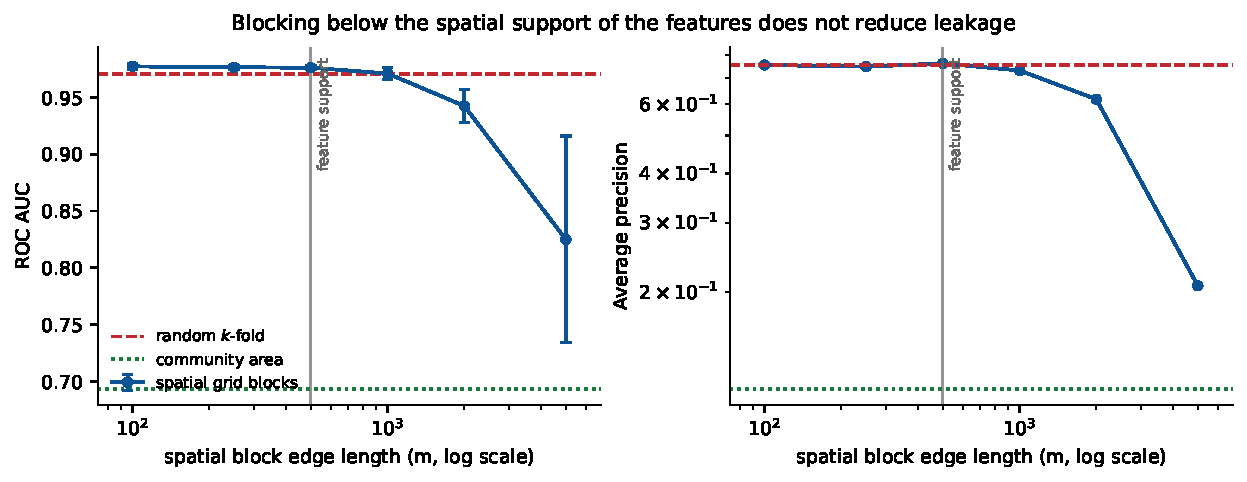
\includegraphics[width=\textwidth]{fig1_block_scale.pdf}
\caption{Performance against spatial block size. The curve is flat until blocks
exceed the $500$\,m spatial support of the features (grey line), then falls.
A practitioner selecting a block below that scale obtains an estimate
indistinguishable from random splits.}
\label{fig:scale}
\end{figure}

Table~\ref{tab:scale} and Figure~\ref{fig:scale} show performance is flat from
random splits through
$1$\,km blocks and falls only beyond $2$\,km. Since features summarise
neighbourhoods to $500$\,m, blocks at or below that scale cannot sever the
dependence they induce: information propagates as far as the blocks are wide.

The practical implication is a diagnostic rather than a fixed recommendation.
Sweeping block size and observing a flat curve indicates blocks are too small
relative to feature support; the curve's decline locates the scale at which
dependence is actually broken.

\subsection{Leakage scales with model capacity}

\begin{table}[t]
\centering
\begin{tabular}{lrrrrr}
\toprule
Model & Random AUC & Blocked AUC & $\Delta$ & Random AP & Blocked AP \\
\midrule
Logistic regression & $0.709$ & $0.696$ & $+0.013$ & $0.098$ & $0.098$ \\
$k$NN ($k=25$)      & $0.686$ & $0.616$ & $+0.070$ & $0.092$ & $0.072$ \\
Random forest       & $0.933$ & $0.686$ & $+0.247$ & $0.670$ & $0.086$ \\
Gradient boosting   & $0.970$ & $0.693$ & $+0.277$ & $0.756$ & $0.114$ \\
\bottomrule
\end{tabular}
\caption{Inflation by model family. Under blocked evaluation all families are
equivalent; under random splits they are not.}
\label{tab:models}
\end{table}

\begin{figure}[t]
\centering
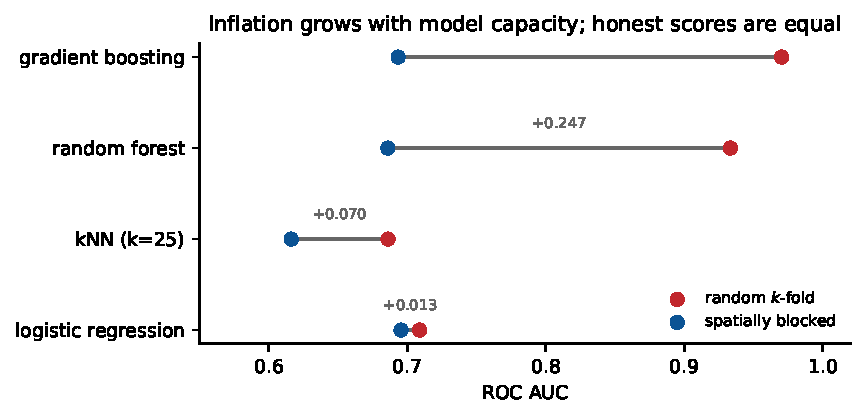
\includegraphics[width=0.78\textwidth]{fig2_model_families.pdf}
\caption{Paired random and blocked scores by model family. Honest scores
coincide; random-split scores do not, so the ranking is an artefact of the
partition.}
\label{fig:models}
\end{figure}

Table~\ref{tab:models} and Figure~\ref{fig:models} show inflation rising with
model flexibility. The
consequence extends beyond reporting. Under random cross-validation gradient
boosting appears to outperform logistic regression by $0.261$ AUC; under blocked
evaluation the gap is $-0.003$. Random splits therefore do not merely inflate a
figure, they invert a model-selection decision, and the inflation is largest
precisely for the model families practitioners most often prefer.

\subsection{Group aggregates dominate the leak}

\begin{table}[t]
\centering
\begin{tabular}{lrrrr}
\toprule
Feature family & $k$ & Random & Blocked & $\Delta$ \\
\midrule
Area aggregates (ward, community area) & 4 & $0.978$ & $0.657$ & $+0.321$ \\
Raw coordinates                        & 2 & $0.659$ & $0.595$ & $+0.064$ \\
Neighbourhood LOO ($50$--$500$\,m)     & 6 & $0.722$ & $0.687$ & $+0.034$ \\
Density counts                         & 3 & $0.694$ & $0.672$ & $+0.021$ \\
Building context                       & 2 & $0.508$ & $0.506$ & $+0.001$ \\
\bottomrule
\end{tabular}
\caption{Inflation by feature family, gradient boosting. Administrative
aggregates inflate an order of magnitude more than proximity features.}
\label{tab:ablation}
\end{table}

\begin{figure}[t]
\centering
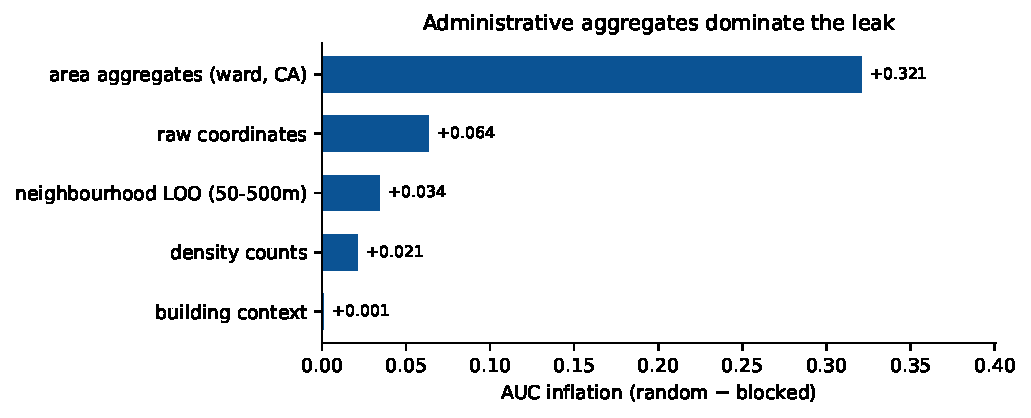
\includegraphics[width=0.78\textwidth]{fig3_feature_ablation.pdf}
\caption{AUC inflation by feature family. Administrative aggregates dominate;
proximity features contribute little.}
\label{fig:ablation}
\end{figure}

Table~\ref{tab:ablation} and Figure~\ref{fig:ablation} localise the leak to
administrative aggregates. Four
features alone reach AUC $0.978$ under random splits and $0.657$ under blocked
splits. Proximity features---the expected culprit---contribute little.

The mechanism is group identity rather than distance. A leave-one-out mean over a
ward is near-constant within that ward, so it serves as a ward identifier; under
a random split, training rows disclose the ward's label rate to test rows in the
same ward. Leave-one-out construction removes the focal observation but not the
remaining $n-1$, and with large groups this is negligible protection.

This reframes the requirement. What must align is not blocks with geography but
\emph{the evaluation partition with the grouping used to construct aggregate
features}. Where those groups are administrative units, spatial blocks of
arbitrary size do not satisfy it. Where the groups are not spatial at all---user,
merchant, session---the same failure arises with no spatial character, and the
same remedy applies.

\subsection{Isolating the mechanism}

The ablation identifies \emph{which} features leak but not \emph{why}, and on
observational data the two are hard to separate: administrative aggregates
differ from neighbourhood features in group size, in spatial extent and in how
strongly their groups differ from one another. We therefore construct encoding
groups directly and vary one property at a time.

Locations are partitioned into $K$ spatial clusters for $K$ between 10 and
4{,}000, giving mean group sizes from 13{,}555 down to 33. For each $K$ we build
a single feature---the leave-one-out group mean of tenant count---and evaluate
it alone, under random folds and under folds aligned with the clusters.

\begin{table}[t]
\centering
\begin{tabular}{rrrrrr}
\toprule
Groups & Mean size & Between-group var. & Random & Group-blocked & $\Delta$ \\
\midrule
   10 & 13{,}555 & $0.00044$ & $0.986$ & $0.571$ & $+0.415$ \\
   25 &  5{,}422 & $0.00036$ & $0.987$ & $0.562$ & $+0.424$ \\
   50 &  2{,}711 & $0.00032$ & $0.943$ & $0.539$ & $+0.404$ \\
  100 &  1{,}355 & $0.00032$ & $0.869$ & $0.487$ & $+0.382$ \\
  250 &     542  & $0.00051$ & $0.803$ & $0.549$ & $+0.254$ \\
 1{,}000 &   135  & $0.00121$ & $0.720$ & $0.563$ & $+0.157$ \\
 4{,}000 &    33  & $0.00364$ & $0.699$ & $0.611$ & $+0.088$ \\
\bottomrule
\end{tabular}
\caption{A single leave-one-out group-mean feature, evaluated under random and
group-aligned folds, as the size of the encoding group varies.}
\label{tab:mechanism}
\end{table}

\begin{figure}[t]
\centering
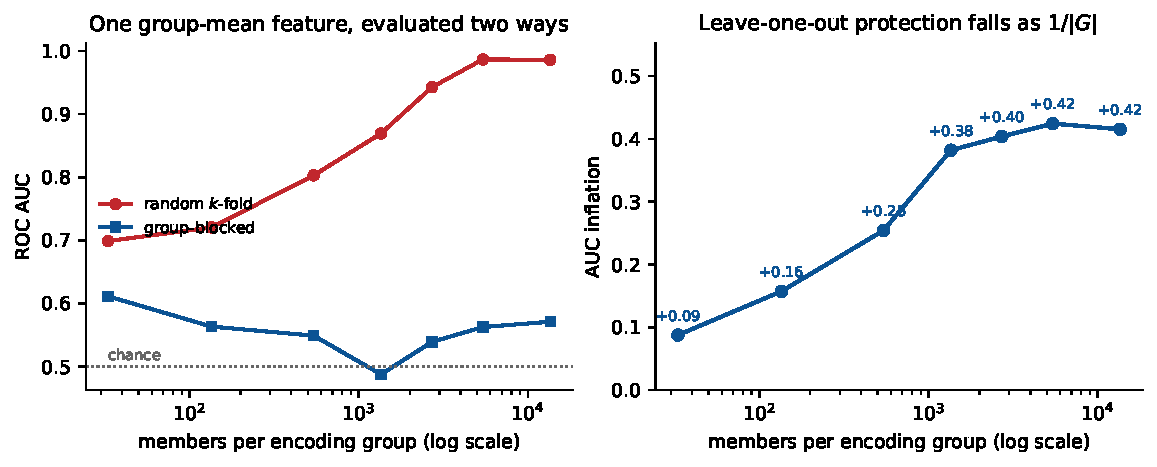
\includegraphics[width=\textwidth]{fig6_mechanism.pdf}
\caption{Leakage against encoding-group size. One feature reaches AUC $0.986$
under random folds while its group-blocked value stays near chance.}
\label{fig:mechanism}
\end{figure}

Three things follow from Table~\ref{tab:mechanism}.

First, the magnitudes are not small. \emph{One} feature reaches AUC $0.986$
under random folds. Nothing else is supplied to the model.

Second, the group-blocked column stays between $0.487$ and $0.611$ throughout.
The feature carries almost no signal that transfers to unseen groups, so
essentially the whole random-fold score is leakage rather than a genuine
relationship that blocking happens to suppress.

Third, inflation tracks group size and not how much the groups differ.
Between-group variance in the label rate rises by a factor of eight as groups
shrink, while inflation falls from $+0.415$ to $+0.088$. Were leakage driven by
groups differing from one another, the two columns would move together; they
move oppositely.

The algebra gives the reason. For a group $G$ the leave-one-out encoding is
\[
f_i \;=\; \frac{1}{|G|-1}\sum_{j \in G,\, j \neq i} y_j
\qquad\text{so}\qquad
f_i \;=\; \bar{y}_G \;+\; \frac{\bar{y}_G - y_i}{|G|-1}.
\]
The encoding differs from the full group mean---the quantity that would leak
$y_i$ outright---by a term of order $1/|G|$. Leave-one-out therefore withholds a
$1/|G|$ share of the signal and no more: about $3\%$ at $|G|=33$, and $0.007\%$
at $|G|=13{,}555$. For large groups it is not a meaningful precaution, and what
remains is a near-constant value within each group, which under random folds
serves as a group identifier whose label rate the training rows disclose.

This accounts for the ablation in Table~\ref{tab:ablation} quantitatively.
Chicago's 50 wards and 78 community areas hold on the order of $1{,}700$
locations each, placing them in the regime where leave-one-out protects almost
nothing; they inflate by $+0.321$. Neighbourhood features at $50$--$500$\,m
aggregate over a handful of premises, where the $1/|G|$ term is substantial;
they inflate by $+0.034$. The distinction is group size, not distance, which is
why partitioning on geometry does not address it.

\subsection{Replication in a second city}

The results so far rest on one city. To test whether they reflect something
general about group-aggregate features or something particular to Chicago's
administrative geography, we rebuilt the task from the New York City Department
of Consumer and Worker Protection licence register (\texttt{w7w3-xahh},
$72{,}452$ records), applying the same address normalisation, the same tenancy
reconstruction and the same succession rule, and supplying the model only with
leave-one-out means over council district, community board and borough.

Finding a second city was itself the obstacle, and the reason is worth
recording. Most municipal portals publish a register of \emph{currently active}
businesses. Seattle's \emph{Active Business License Tax Certificate} carries a
start date and no end date; Los Angeles's \emph{Listing of Active Businesses}
has an end-date column that is null in all $631{,}925$ rows. Neither permits
closure to be observed at all. Chicago's practice of publishing every licence
issued since 1995, with cancellation dates, is unusual, and it is why this
analysis has a thirty-year window in one city and a much shorter one elsewhere.

\begin{table}[t]
\centering
\begin{tabular}{lrr}
\toprule
 & Chicago & New York \\
\midrule
Licence records            & $1{,}207{,}055$ & $72{,}452$ \\
Locations                  & $161{,}607$ & $40{,}964$ \\
Multi-tenant locations     & $24{,}383$ ($15\%$) & $813$ ($2\%$) \\
Maximum tenants at one address & $20$ & $3$ \\
Administrative groups      & $78$ & $52$ \\
\midrule
Random $k$-fold AUC        & $0.978$ & $0.651$ \\
Group-blocked AUC          & $0.657$ & $0.581$ \\
Inflation                  & $+0.321$ & $+0.070$ \\
\bottomrule
\end{tabular}
\caption{Group-aggregate features evaluated identically in both cities. The
direction reproduces; the magnitude does not.}
\label{tab:nyc}
\end{table}

Table~\ref{tab:nyc} shows leakage in the same direction in New York, at roughly
one fifth of the Chicago magnitude. We take this as a boundary condition rather
than a confirmation, and the mechanism of Section~5.4 predicts it.

A group mean can only leak to the extent that it varies between groups, and that
variation comes from the outcome. New York's register begins in 2019 rather than
1995, so $98\%$ of its locations have a single tenant and the maximum is three.
The group means are therefore nearly constant across the city, and carry little
to encode. Chicago's thirty-year window produces $15\%$ multi-tenant locations
and turnover counts up to $20$, giving the same features far more group-level
structure to transmit.

The claim this supports is accordingly narrower than "group aggregates leak
everywhere". It is that leakage through group aggregates scales with how much
group-level structure the outcome carries, and that where it is substantial---as
in a register deep enough to observe real turnover---spatial blocking does not
remove it. A shallow register understates the hazard; it does not make it safe,
since the practitioner cannot tell from the inflated number which regime they
are in.

\subsection{The substantive finding}

Under honest evaluation the urban result stands. Excess turnover concentrates at
individual addresses rather than districts. Leave-one-out neighbour turnover
exceeds the within-area permutation null by $+0.104$ tenants at $50$\,m
($p = 0.001$, null $+0.034 \pm 0.003$), $+0.068$ at $200$\,m and $+0.040$ at
$500$\,m, against a focal difference of $+1.99$ tenants. Neighbours of
high-turnover addresses are elevated by roughly $5\%$; the addresses themselves
by roughly $176\%$.

\begin{figure}[t]
\centering
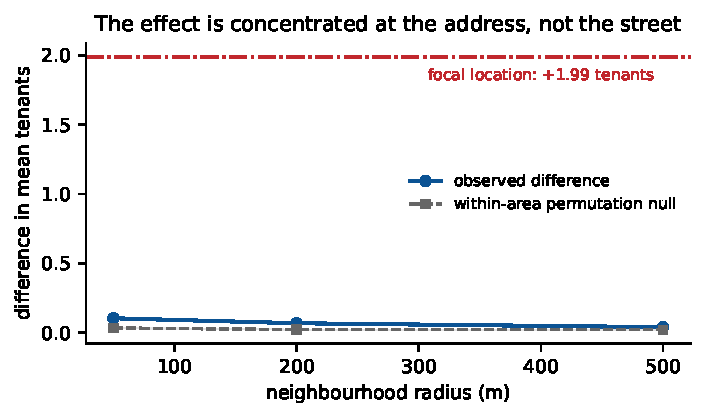
\includegraphics[width=\textwidth]{fig5_neighbour_decay.pdf}
\caption{Difference in mean tenant count between high-turnover locations and the
remainder, by neighbourhood radius, against a permutation null that shuffles
labels within community areas. The focal difference exceeds the neighbour
difference by an order of magnitude.}
\label{fig:decay}
\end{figure}

\begin{figure}[t]
\centering
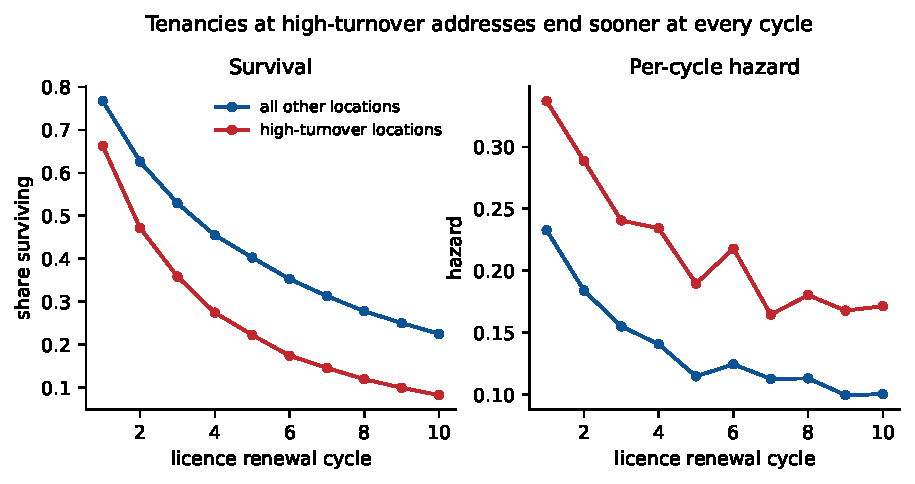
\includegraphics[width=\textwidth]{fig4_survival.pdf}
\caption{Discrete-time survival and per-cycle hazard over licence renewal
cycles. Renewal cycles are used in place of elapsed days because duration is
quantized to licence terms.}
\label{fig:survival}
\end{figure}

Discrete-time survival over renewal cycles (Figure~\ref{fig:survival}) shows
tenancies at these locations
ending faster at every stage: first-cycle hazard $0.337$ against $0.233$, and
survival to the eighth cycle of $0.119$ against $0.278$. The hazard ratio is
approximately constant across cycles, consistent with proportional hazards.

Context predicts the label only weakly (AUC $0.693$, AP $2.3\times$ base rate).
Most excess turnover is therefore not explained by observable surroundings.

\subsection{Sensitivity to the target definition}

\begin{table}[t]
\centering
\begin{tabular}{lrrr}
\toprule
 & Count & Rate & Excess \\
\midrule
Count ($\geq 4$ tenants)        & $1.000$ & $0.187$ & $0.193$ \\
Rate (tenants per decade, top $5\%$) & $0.187$ & $1.000$ & $0.632$ \\
Excess (model residual, top $5\%$)   & $0.193$ & $0.632$ & $1.000$ \\
\bottomrule
\end{tabular}
\caption{Jaccard overlap between the sets of locations flagged by three target
definitions.}
\label{tab:definitions}
\end{table}

Table~\ref{tab:definitions} reports agreement between the three definitions.
The exposure-adjusted definitions overlap substantially (Jaccard $0.632$), but
the unadjusted count-based definition overlaps both only weakly ($0.187$,
$0.193$). This is a genuine limitation and we state it plainly: which addresses
are called high-turnover depends materially on whether exposure and sector are
adjusted for, and a reader who prefers a raw-count definition would be studying
a substantially different set of locations.

This sensitivity concerns the substantive finding rather than the evaluation
findings, and we verify rather than assume the distinction. Repeating the
random-versus-blocked comparison under each definition gives inflations of
$+0.340$ (count), $+0.305$ (rate) and $+0.295$ (excess), with random-fold AUC
between $0.951$ and $0.977$ and blocked AUC between $0.637$ and $0.676$. The
three definitions select substantially different locations, yet the leakage they
exhibit is the same to within $0.045$ AUC. The evaluation findings are therefore
invariant to a choice that materially changes the substantive one, as the
mechanism implies: leakage depends on how the features are constructed, not on
how the label is defined.

\section{Recommendations}

\begin{enumerate}
\item \textbf{Partition by the grouping used for aggregate features.} If features
include group-level statistics, folds must respect those groups. This subsumes
spatial blocking when groups are geographic and applies unchanged when they are
not.
\item \textbf{Report a block-size sweep.} A flat performance curve across block
sizes indicates blocks below feature support. The curve costs little and makes
the claim auditable.
\item \textbf{Treat leave-one-out as insufficient.} It removes the focal
observation only. With large groups the remaining members carry essentially the
full signal.
\item \textbf{Compare model families under the final protocol.} Capacity-dependent
inflation means selection under random splits can invert under blocked splits.
\item \textbf{Report average precision with the base rate} for imbalanced targets.
\end{enumerate}

\section{Limitations}

Licence records proxy trading. A lapse may reflect administrative change rather
than closure; our succession merge is a conservative but imperfect correction,
and residual misclassification inflates apparent turnover.

Duration is interval-censored and quantized, which is why we use renewal cycles;
absolute tenure figures should not be read from this data.

Community area enters both the target definition and the partitioning, so
area-level comparisons are circular and excluded from substantive claims.

The urban finding rests on Chicago alone. Our New York replication speaks to
the evaluation results, not to the turnover result, whose magnitude that register
is too shallow to measure. Whether high-turnover addresses concentrate similarly
in other cities is untested, and testing it requires registers that record
closure, which most cities do not publish.

Excess turnover is defined relative to a model, so the label inherits that
model's assumptions. Three alternative definitions are reported in the
supplement.

\section{Conclusion}

Spatial blocking and group-aware partitioning address different hazards, and in
urban prediction both are usually present at once. When features include
aggregates over administrative units, the dominant leakage channel is group
membership rather than proximity, and spatial blocks do not close it until they
approach the size of those units---well beyond the scale current block-size
guidance would suggest. On our task the difference between the default protocol
and a correct one is ROC AUC $0.970$ against $0.693$, average precision inflated
more than sixfold, and a reversal of model selection.

The practical consequence is narrow but, we think, worth stating: a practitioner
who identifies their data as spatial, adopts spatial cross-validation and sets
block size from predictor autocorrelation has done everything the spatial
literature asks and still obtains a fully inflated estimate. The check that would
have caught it is cheap---sweep the block size and look for a flat curve---and
the fix is to partition by the units the features aggregate over.

The effect is bounded rather than universal. A second city reproduces it in
direction at roughly one fifth the magnitude, because its register is too
shallow for much turnover to have been observed and group means with little
variance have little to transmit. Leakage through group aggregates therefore
scales with the group-level structure the outcome carries. That is a weaker
claim than "group aggregates always leak", and a more useful one: it says where
to look, and it means a modest inflation in a shallow dataset is not evidence of
safety.

The substantive finding survives honest evaluation: excess commercial turnover
concentrates at individual addresses rather than districts, with immediate
neighbours only weakly elevated, and tenancies at such addresses ending roughly
$1.5\times$ faster per renewal cycle.

\section*{Acknowledgements}

The authors thank Huanyu Li for supervision and guidance. Responsibility for the
analysis and for any errors rests with the authors.

\section*{Reproducibility}

All inputs are public domain: the licence register is published by the City of
Chicago as dataset \texttt{r5kz-chrr} and may be retrieved by anyone. Section~3
states the extraction date, the row count against which the download was
verified, and every threshold used to reconstruct tenancies, so the derived
tables can be rebuilt from the published source.

The analysis code, the download utility with row-count verification, and the
derived tenancy and location tables are released at
\begin{center}
\url{https://github.com/naazzarov/storefront-turnover-leakage}
\end{center}
A single entry point, \texttt{run\_experiments.py}, regenerates every table and
figure in one pass, and the pipeline is deterministic given the seed recorded in
the repository.

\bibliographystyle{plainnat}
\begin{thebibliography}{99}

\bibitem[Dunne et al.(1988)]{dunne1988}
T.~Dunne, M.~J. Roberts, and L.~Samuelson.
\newblock Patterns of firm entry and exit in U.S. manufacturing industries.
\newblock \emph{RAND Journal of Economics}, 19(4):495--515, 1988.

\bibitem[Stock(2025)]{stock2025}
A.~Stock.
\newblock Choosing blocks for spatial cross-validation: lessons from a marine
  remote sensing case study.
\newblock \emph{Frontiers in Remote Sensing}, 6, 2025.
\newblock \url{https://doi.org/10.3389/frsen.2025.1531097}.

\bibitem[Rosenblatt et al.(2024)]{rosenblatt2024}
M.~Rosenblatt, L.~Tejavibulya, R.~Jiang, S.~Noble, and D.~Scheinost.
\newblock Data leakage inflates prediction performance in connectome-based
  machine learning models.
\newblock \emph{Nature Communications}, 15, 2024.
\newblock \url{https://doi.org/10.1038/s41467-024-46150-w}.

\bibitem[Cerqua et al.(2024)]{misuse2024}
A.~Cerqua, M.~Letta, and G.~Pinto.
\newblock On the (mis)use of machine learning with panel data.
\newblock \emph{arXiv preprint arXiv:2411.09218}, 2024.

\bibitem[Kapoor and Narayanan(2023)]{kapoor2023}
S.~Kapoor and A.~Narayanan.
\newblock Leakage and the reproducibility crisis in machine-learning-based
  science.
\newblock \emph{Patterns}, 4(9), 2023.

\bibitem[Kaufman et al.(2012)]{kaufman2012}
S.~Kaufman, S.~Rosset, C.~Perlich, and O.~Stitelman.
\newblock Leakage in data mining: Formulation, detection, and avoidance.
\newblock \emph{ACM TKDD}, 6(4):1--21, 2012.

\bibitem[Micci-Barreca(2001)]{micci2001}
D.~Micci-Barreca.
\newblock A preprocessing scheme for high-cardinality categorical attributes in
  classification and prediction problems.
\newblock \emph{ACM SIGKDD Explorations}, 3(1):27--32, 2001.

\bibitem[Ploton et al.(2020)]{ploton2020}
P.~Ploton et al.
\newblock Spatial validation reveals poor predictive performance of large-scale
  ecological mapping models.
\newblock \emph{Nature Communications}, 11:4540, 2020.

\bibitem[Prokhorenkova et al.(2018)]{prokhorenkova2018}
L.~Prokhorenkova, G.~Gusev, A.~Vorobev, A.~V. Dorogush, and A.~Gulin.
\newblock CatBoost: unbiased boosting with categorical features.
\newblock In \emph{NeurIPS}, 2018.

\bibitem[Roberts et al.(2017)]{roberts2017}
D.~R. Roberts et al.
\newblock Cross-validation strategies for data with temporal, spatial,
  hierarchical, or phylogenetic structure.
\newblock \emph{Ecography}, 40(8):913--929, 2017.

\bibitem[Valavi et al.(2019)]{valavi2019}
R.~Valavi, J.~Elith, J.~J. Lahoz-Monfort, and G.~Guillera-Arroita.
\newblock blockCV: An R package for generating spatially or environmentally
  separated folds.
\newblock \emph{Methods in Ecology and Evolution}, 10(2):225--232, 2019.

\end{thebibliography}

\end{document}
